\clearpage\SourceLeaf{353}

\begin{center}[\emph{Vorlesung über die Theorie der imaginären Grössen.}]\end{center}

\begin{center}\bfseries Projection des Würfels.\end{center}

Will man einen Würfel auf eine Ebene projiciren, und zwar durch Senkrechte von den Ecken auf die Ebene, so muss die Projection die Eigenschaft haben, dass die Summe der Quadrate der Zahlen, die die Projection je dreier auf einander stossender Kanten anzeigen, $=0$ sei.

Um diess zu zeigen, bezeichnen wir mit $0,1,7,3$ die Ecken der einen, mit $2,4,5,6$ die der damit parallelen Fläche. Ist $(0,1)$, die Seite des Würfels, $=r$, so haben wir, dass an der Ecke $0$ die drei Kanten zusammenstossen, deren jede $=r$ ist:

\begin{center}\resizebox{4.6cm}{!}{%
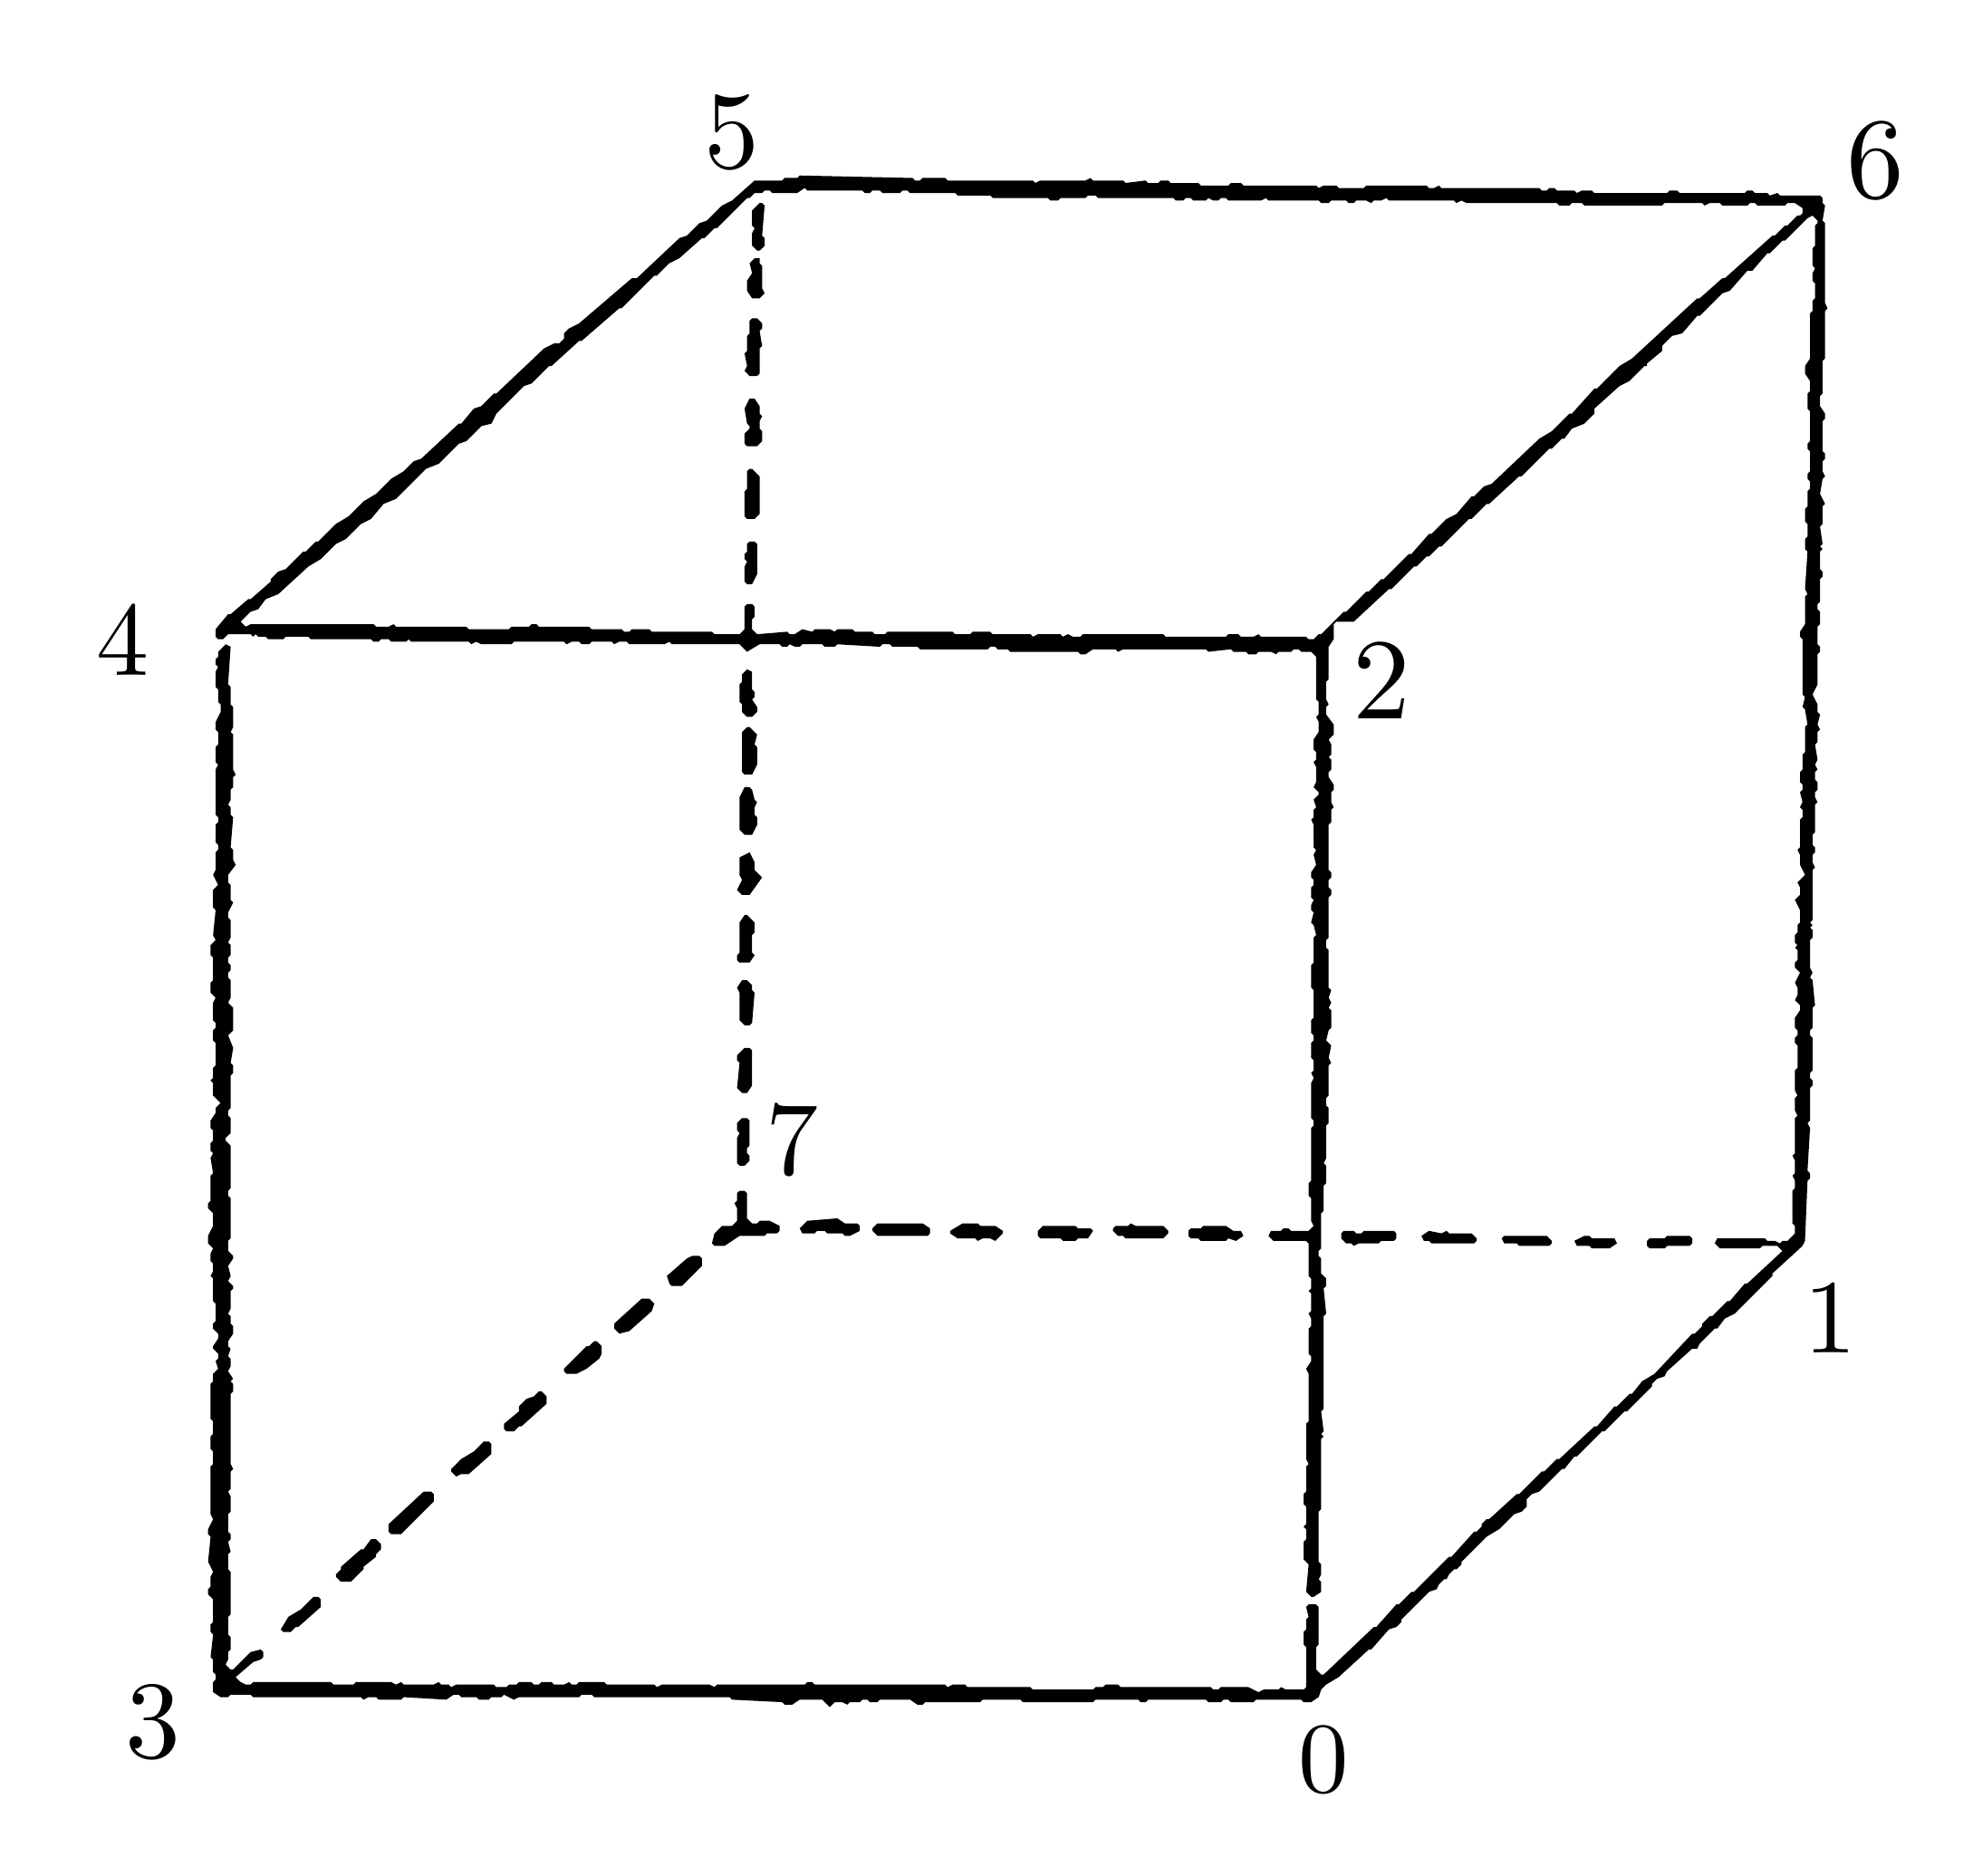
\begin{tikzpicture}[x=1pt,y=-1pt]
\path[use as bounding box] (0,0) rectangle (767,728);
\path[fill=black,draw=none,even odd rule]
(118,628) -- (117,627) -- (115,627) -- (110,632) -- (105,635) -- (102,640) -- (103,641) -- (106,641) -- (108,639) -- (109,639) -- (118,631) -- cycle
(140,604) -- (138,604) -- (135,608) -- (134,608) -- (126,615) -- (126,616) -- (124,618) -- (124,619) -- (126,621) -- (130,621) -- (135,616) -- (135,615) -- (140,611) -- (140,610) -- (142,608) -- (142,606) -- cycle
(163,586) -- (162,585) -- (159,585) -- (145,598) -- (145,601) -- (146,602) -- (150,602) -- (163,589) -- cycle
(186,566) -- (185,565) -- (183,565) -- (179,569) -- (174,572) -- (170,576) -- (170,577) -- (172,579) -- (174,578) -- (177,578) -- (186,570) -- cycle
(208,547) -- (206,545) -- (205,545) -- (203,547) -- (200,548) -- (197,551) -- (197,553) -- (191,558) -- (191,560) -- (192,561) -- (195,561) -- (197,559) -- (198,559) -- (208,550) -- cycle
(230,527) -- (228,525) -- (227,525) -- (225,527) -- (224,527) -- (215,536) -- (215,537) -- (216,538) -- (220,538) -- (224,536) -- (229,532) -- (230,530) -- cycle
(251,510) -- (249,508) -- (246,508) -- (235,518) -- (235,520) -- (237,522) -- (241,521) -- (250,513) -- cycle
(270,492) -- (269,491) -- (266,491) -- (264,492) -- (256,499) -- (257,502) -- (258,503) -- (262,503) -- (270,495) -- cycle
(647,485) -- (647,487) -- (648,488) -- (654,488) -- (655,487) -- (664,487) -- (665,486) -- (665,484) -- (664,483) -- (655,483) -- (654,484) -- (648,484) -- cycle
(618,485) -- (619,487) -- (624,487) -- (625,488) -- (632,488) -- (635,486) -- (634,484) -- (625,484) -- (624,483) -- (622,483) -- cycle
(589,484) -- (590,486) -- (595,486) -- (596,487) -- (608,487) -- (609,486) -- (609,485) -- (607,483) -- (590,483) -- cycle
(557,483) -- (558,485) -- (560,485) -- (561,486) -- (578,486) -- (579,485) -- (579,484) -- (577,482) -- (568,482) -- (567,481) -- (565,482) -- (560,481) -- cycle
(525,482) -- (525,484) -- (527,486) -- (529,486) -- (530,487) -- (532,486) -- (540,486) -- (541,485) -- (546,485) -- (547,484) -- (547,482) -- (546,481) -- (534,481) -- (533,482) -- (531,482) -- (530,481) -- (526,481) -- cycle
(464,481) -- (464,483) -- (465,484) -- (468,484) -- (469,485) -- (479,485) -- (480,484) -- (483,485) -- (486,483) -- (485,481) -- (482,481) -- (479,479) -- (470,479) -- (469,480) -- (465,480) -- cycle
(404,483) -- (405,484) -- (413,484) -- (414,485) -- (419,485) -- (420,484) -- (424,484) -- (426,481) -- (425,480) -- (420,480) -- (419,479) -- (406,479) -- (404,481) -- cycle
(434,480) -- (434,481) -- (436,483) -- (438,483) -- (439,484) -- (454,484) -- (456,482) -- (456,481) -- (454,479) -- (443,479) -- (441,478) -- (440,479) -- (435,479) -- cycle
(369,481) -- (369,482) -- (372,484) -- (379,484) -- (380,485) -- (382,484) -- (385,484) -- (387,485) -- (390,482) -- (390,481) -- (387,479) -- (381,479) -- (380,478) -- (374,478) -- cycle
(338,480) -- (338,481) -- (340,483) -- (360,483) -- (361,482) -- (361,480) -- (358,478) -- (340,478) -- cycle
(309,480) -- (310,482) -- (315,482) -- (316,481) -- (319,481) -- (320,482) -- (326,482) -- (327,483) -- (329,483) -- (333,481) -- (333,479) -- (332,478) -- (327,478) -- (324,476) -- (312,477) -- cycle
(301,479) -- (297,477) -- (293,477) -- (292,478) -- (290,478) -- (288,476) -- (288,466) -- (287,465) -- (285,465) -- (284,466) -- (284,469) -- (283,470) -- (284,472) -- (284,477) -- (282,479) -- (278,479) -- (275,482) -- (274,486) -- (275,487) -- (279,487) -- (285,483) -- (295,483) -- (296,482) -- (300,482) -- (301,481) -- cycle
(288,436) -- (286,436) -- (284,438) -- (284,441) -- (285,442) -- (284,444) -- (284,454) -- (285,455) -- (287,455) -- (289,453) -- (289,451) -- (288,450) -- (288,448) -- (289,447) -- (289,437) -- cycle
(289,408) -- (287,408) -- (284,411) -- (284,413) -- (285,414) -- (284,424) -- (286,426) -- (288,426) -- (290,423) -- (290,409) -- cycle
(286,381) -- (284,384) -- (285,386) -- (285,397) -- (287,399) -- (289,399) -- (290,398) -- (291,386) -- (290,385) -- (290,383) -- (288,381) -- cycle
(288,355) -- (287,355) -- (285,358) -- (285,370) -- (284,371) -- (284,373) -- (285,374) -- (289,374) -- (291,371) -- (290,370) -- (290,363) -- (291,362) -- (291,358) -- cycle
(289,330) -- (285,332) -- (285,339) -- (286,341) -- (284,345) -- (286,347) -- (289,347) -- (294,340) -- (291,337) -- (291,334) -- cycle
(287,304) -- (285,308) -- (285,321) -- (287,323) -- (290,323) -- (292,319) -- (292,316) -- (291,315) -- (291,312) -- (292,310) -- (291,309) -- (290,305) -- (289,304) -- cycle
(288,280) -- (286,282) -- (286,298) -- (287,299) -- (290,299) -- (292,295) -- (292,288) -- (291,287) -- (292,283) -- (289,280) -- cycle
(288,257) -- (286,259) -- (286,262) -- (285,263) -- (285,270) -- (286,271) -- (286,274) -- (288,276) -- (290,276) -- (292,274) -- (292,272) -- (290,269) -- (291,268) -- (291,266) -- (290,265) -- (290,258) -- cycle
(717,69) -- (716,68) -- (700,68) -- (699,67) -- (696,68) -- (695,67) -- (690,67) -- (689,66) -- (687,66) -- (686,67) -- (660,67) -- (659,66) -- (656,66) -- (655,67) -- (626,67) -- (625,66) -- (621,66) -- (619,67) -- (618,66) -- (611,66) -- (610,65) -- (608,65) -- (607,66) -- (605,66) -- (604,65) -- (565,65) -- (564,64) -- (562,65) -- (560,65) -- (559,64) -- (535,64) -- (534,65) -- (524,65) -- (523,64) -- (518,64) -- (516,65) -- (515,64) -- (486,64) -- (485,63) -- (481,63) -- (480,64) -- (469,64) -- (468,63) -- (457,63) -- (456,62) -- (453,62) -- (452,63) -- (448,63) -- (447,62) -- (439,63) -- (438,62) -- (426,62) -- (425,61) -- (423,62) -- (405,62) -- (403,63) -- (402,62) -- (368,62) -- (367,61) -- (358,61) -- (357,62) -- (355,62) -- (354,61) -- (309,60) -- (308,61) -- (303,61) -- (302,62) -- (291,62) -- (282,70) -- (278,72) -- (272,78) -- (269,79) -- (264,84) -- (261,85) -- (244,101) -- (242,101) -- (221,119) -- (217,121) -- (215,123) -- (215,125) -- (213,127) -- (211,127) -- (207,129) -- (188,147) -- (187,147) -- (182,152) -- (179,153) -- (174,159) -- (173,159) -- (158,173) -- (155,174) -- (151,178) -- (146,181) -- (140,187) -- (135,190) -- (129,196) -- (124,199) -- (117,206) -- (116,206) -- (112,210) -- (111,210) -- (104,217) -- (101,218) -- (98,221) -- (98,222) -- (90,229) -- (89,229) -- (82,235) -- (81,235) -- (76,241) -- (76,244) -- (77,245) -- (79,245) -- (81,243) -- (90,243) -- (91,244) -- (92,243) -- (93,244) -- (96,244) -- (97,245) -- (103,245) -- (104,244) -- (113,244) -- (114,245) -- (138,245) -- (139,246) -- (141,246) -- (142,245) -- (145,245) -- (146,246) -- (152,246) -- (153,245) -- (154,246) -- (177,246) -- (178,247) -- (180,246) -- (182,247) -- (194,247) -- (195,246) -- (215,246) -- (216,247) -- (218,246) -- (221,246) -- (222,247) -- (225,247) -- (226,246) -- (234,246) -- (235,247) -- (237,246) -- (240,246) -- (241,247) -- (255,247) -- (257,246) -- (258,247) -- (285,247) -- (288,250) -- (293,247) -- (301,247) -- (302,248) -- (304,248) -- (305,247) -- (307,248) -- (309,248) -- (310,247) -- (318,247) -- (319,248) -- (323,248) -- (324,247) -- (341,248) -- (342,247) -- (345,247) -- (346,248) -- (356,248) -- (357,249) -- (384,249) -- (385,248) -- (387,248) -- (388,249) -- (392,249) -- (393,250) -- (420,250) -- (421,251) -- (423,251) -- (426,249) -- (435,249) -- (436,250) -- (438,249) -- (471,249) -- (472,250) -- (481,249) -- (482,250) -- (487,250) -- (488,251) -- (491,251) -- (492,250) -- (497,250) -- (499,251) -- (500,250) -- (505,250) -- (506,249) -- (508,249) -- (509,250) -- (513,250) -- (515,252) -- (515,269) -- (516,270) -- (516,275) -- (515,276) -- (516,278) -- (516,282) -- (514,285) -- (514,289) -- (515,290) -- (515,293) -- (514,294) -- (515,296) -- (515,302) -- (514,304) -- (516,306) -- (516,307) -- (514,309) -- (515,312) -- (514,313) -- (514,316) -- (513,317) -- (514,319) -- (514,328) -- (515,329) -- (514,331) -- (515,335) -- (513,338) -- (513,340) -- (514,341) -- (514,343) -- (513,344) -- (513,348) -- (514,349) -- (513,351) -- (513,353) -- (514,354) -- (513,358) -- (514,359) -- (515,363) -- (514,364) -- (514,374) -- (513,375) -- (513,384) -- (514,385) -- (514,396) -- (513,397) -- (513,402) -- (514,403) -- (514,405) -- (513,406) -- (513,412) -- (514,413) -- (514,417) -- (513,418) -- (514,420) -- (513,422) -- (513,436) -- (514,437) -- (514,439) -- (513,440) -- (513,461) -- (512,462) -- (512,467) -- (513,468) -- (513,477) -- (514,479) -- (512,481) -- (505,481) -- (504,480) -- (502,480) -- (501,481) -- (497,481) -- (496,483) -- (498,485) -- (511,485) -- (512,486) -- (512,499) -- (513,500) -- (513,504) -- (512,505) -- (513,506) -- (513,513) -- (512,514) -- (513,516) -- (513,519) -- (512,520) -- (512,530) -- (513,531) -- (513,533) -- (511,536) -- (512,538) -- (512,557) -- (511,558) -- (511,572) -- (512,574) -- (511,575) -- (511,585) -- (510,586) -- (510,590) -- (511,591) -- (511,598) -- (510,599) -- (511,600) -- (511,604) -- (510,605) -- (510,612) -- (512,614) -- (511,625) -- (513,627) -- (514,627) -- (517,625) -- (517,621) -- (516,620) -- (517,618) -- (517,614) -- (516,613) -- (516,593) -- (517,592) -- (517,564) -- (518,563) -- (517,562) -- (518,561) -- (517,553) -- (518,552) -- (518,515) -- (519,514) -- (518,504) -- (519,503) -- (519,500) -- (517,498) -- (517,492) -- (516,491) -- (516,489) -- (517,488) -- (517,474) -- (518,473) -- (518,463) -- (519,462) -- (519,455) -- (518,454) -- (519,452) -- (519,439) -- (520,438) -- (520,432) -- (519,431) -- (519,428) -- (520,427) -- (520,415) -- (521,414) -- (520,412) -- (521,407) -- (519,405) -- (520,401) -- (521,400) -- (521,393) -- (520,392) -- (521,390) -- (520,388) -- (521,385) -- (520,384) -- (520,369) -- (519,368) -- (519,365) -- (520,364) -- (520,348) -- (521,347) -- (521,345) -- (520,344) -- (520,341) -- (521,340) -- (521,338) -- (520,337) -- (520,319) -- (521,318) -- (521,313) -- (522,312) -- (521,310) -- (521,306) -- (522,305) -- (522,303) -- (520,300) -- (520,298) -- (521,297) -- (521,293) -- (520,292) -- (521,291) -- (521,287) -- (520,285) -- (522,283) -- (522,279) -- (519,275) -- (519,272) -- (520,271) -- (519,269) -- (519,262) -- (520,261) -- (520,248) -- (522,245) -- (522,239) -- (523,238) -- (530,238) -- (544,225) -- (545,225) -- (554,216) -- (555,216) -- (559,212) -- (560,212) -- (564,208) -- (565,208) -- (576,197) -- (577,197) -- (583,191) -- (584,191) -- (596,180) -- (597,180) -- (608,169) -- (609,169) -- (613,165) -- (614,165) -- (617,161) -- (622,159) -- (626,155) -- (626,153) -- (636,144) -- (640,142) -- (646,136) -- (647,136) -- (647,135) -- (653,130) -- (653,128) -- (657,124) -- (661,123) -- (667,116) -- (668,116) -- (677,107) -- (680,106) -- (687,98) -- (689,98) -- (695,91) -- (696,91) -- (701,86) -- (702,86) -- (711,77) -- (713,76) -- (715,78) -- (715,79) -- (714,80) -- (714,88) -- (713,89) -- (713,96) -- (714,97) -- (713,99) -- (713,102) -- (714,103) -- (714,109) -- (713,110) -- (713,114) -- (712,115) -- (712,133) -- (710,136) -- (710,139) -- (712,142) -- (712,146) -- (711,147) -- (711,153) -- (712,154) -- (712,166) -- (711,167) -- (711,169) -- (712,170) -- (712,178) -- (711,179) -- (711,181) -- (712,182) -- (712,185) -- (711,186) -- (711,192) -- (710,193) -- (710,198) -- (711,199) -- (711,204) -- (710,205) -- (710,209) -- (711,210) -- (710,225) -- (711,227) -- (710,228) -- (710,239) -- (708,242) -- (708,244) -- (709,245) -- (709,267) -- (710,268) -- (709,272) -- (710,273) -- (711,279) -- (710,280) -- (710,290) -- (709,291) -- (709,297) -- (708,298) -- (708,302) -- (709,303) -- (709,305) -- (708,306) -- (709,310) -- (708,312) -- (709,313) -- (709,316) -- (708,317) -- (708,328) -- (707,329) -- (708,331) -- (708,335) -- (710,339) -- (707,342) -- (708,344) -- (708,347) -- (706,349) -- (708,353) -- (708,358) -- (707,359) -- (707,362) -- (706,363) -- (706,366) -- (707,367) -- (706,368) -- (707,369) -- (707,373) -- (706,374) -- (706,376) -- (708,378) -- (706,382) -- (707,384) -- (707,387) -- (706,389) -- (708,391) -- (708,393) -- (706,396) -- (706,400) -- (707,401) -- (707,403) -- (706,404) -- (706,406) -- (707,407) -- (707,416) -- (706,417) -- (706,425) -- (707,427) -- (706,428) -- (706,433) -- (707,435) -- (706,436) -- (706,450) -- (705,451) -- (706,453) -- (706,458) -- (705,459) -- (706,461) -- (706,464) -- (705,465) -- (705,478) -- (706,479) -- (706,482) -- (703,485) -- (701,485) -- (700,486) -- (698,485) -- (695,485) -- (694,484) -- (675,484) -- (674,486) -- (676,488) -- (692,488) -- (693,487) -- (699,487) -- (701,489) -- (687,502) -- (686,502) -- (680,509) -- (679,509) -- (673,515) -- (672,515) -- (669,518) -- (669,519) -- (666,522) -- (665,522) -- (650,538) -- (645,541) -- (641,546) -- (640,546) -- (635,551) -- (634,551) -- (627,559) -- (626,559) -- (612,572) -- (611,572) -- (606,577) -- (605,577) -- (596,586) -- (595,586) -- (584,596) -- (583,596) -- (581,598) -- (581,599) -- (579,601) -- (578,601) -- (569,611) -- (568,611) -- (554,625) -- (553,625) -- (548,630) -- (547,630) -- (539,639) -- (538,639) -- (518,658) -- (517,658) -- (515,656) -- (515,647) -- (516,646) -- (516,631) -- (515,630) -- (512,630) -- (511,631) -- (512,635) -- (511,636) -- (511,640) -- (510,641) -- (510,646) -- (511,647) -- (511,663) -- (510,664) -- (503,664) -- (501,663) -- (500,664) -- (494,664) -- (492,665) -- (488,663) -- (477,663) -- (476,664) -- (474,664) -- (473,663) -- (437,663) -- (436,662) -- (431,662) -- (430,663) -- (427,663) -- (426,664) -- (402,664) -- (401,663) -- (376,663) -- (375,662) -- (370,662) -- (368,663) -- (367,662) -- (315,662) -- (314,661) -- (312,661) -- (311,662) -- (276,662) -- (275,663) -- (273,662) -- (254,662) -- (252,663) -- (251,662) -- (232,662) -- (231,661) -- (221,661) -- (220,662) -- (218,662) -- (217,661) -- (215,662) -- (211,662) -- (210,661) -- (206,661) -- (205,662) -- (203,662) -- (202,661) -- (197,661) -- (196,662) -- (193,662) -- (192,663) -- (188,663) -- (187,662) -- (172,662) -- (170,663) -- (169,662) -- (166,662) -- (165,661) -- (163,662) -- (151,662) -- (150,661) -- (148,662) -- (146,661) -- (132,661) -- (131,662) -- (123,662) -- (122,661) -- (91,661) -- (90,662) -- (88,662) -- (86,661) -- (84,659) -- (91,653) -- (94,652) -- (95,651) -- (95,649) -- (94,648) -- (90,649) -- (83,656) -- (82,656) -- (80,654) -- (81,652) -- (81,649) -- (82,648) -- (82,643) -- (81,642) -- (81,635) -- (82,634) -- (82,617) -- (81,616) -- (81,610) -- (82,609) -- (81,605) -- (82,604) -- (82,602) -- (81,601) -- (81,594) -- (82,593) -- (82,587) -- (81,585) -- (82,584) -- (82,577) -- (83,576) -- (82,574) -- (82,546) -- (83,545) -- (83,542) -- (82,541) -- (83,540) -- (81,537) -- (82,535) -- (82,532) -- (81,531) -- (82,528) -- (81,527) -- (81,525) -- (83,522) -- (83,519) -- (82,518) -- (82,515) -- (81,514) -- (82,512) -- (82,505) -- (83,504) -- (83,503) -- (81,501) -- (82,499) -- (81,495) -- (83,492) -- (83,491) -- (81,489) -- (81,485) -- (82,484) -- (82,468) -- (81,467) -- (81,465) -- (82,464) -- (82,447) -- (80,445) -- (80,444) -- (82,442) -- (82,436) -- (81,435) -- (81,433) -- (82,432) -- (82,419) -- (83,418) -- (83,415) -- (82,414) -- (83,408) -- (81,403) -- (83,401) -- (83,392) -- (81,390) -- (82,388) -- (82,381) -- (81,380) -- (81,378) -- (82,377) -- (82,375) -- (81,374) -- (81,372) -- (82,371) -- (82,367) -- (81,366) -- (82,364) -- (82,357) -- (81,356) -- (81,354) -- (83,350) -- (82,349) -- (82,343) -- (81,342) -- (81,339) -- (84,335) -- (83,333) -- (83,329) -- (82,328) -- (83,316) -- (82,315) -- (82,312) -- (81,311) -- (82,309) -- (82,305) -- (83,304) -- (83,300) -- (84,299) -- (83,297) -- (83,283) -- (82,282) -- (83,280) -- (83,272) -- (82,271) -- (82,264) -- (81,263) -- (82,248) -- (80,247) -- (77,250) -- (77,252) -- (76,253) -- (76,255) -- (77,256) -- (76,258) -- (76,264) -- (77,265) -- (77,270) -- (78,271) -- (78,274) -- (76,278) -- (76,281) -- (77,282) -- (77,287) -- (76,288) -- (76,294) -- (77,295) -- (76,297) -- (76,315) -- (77,316) -- (77,318) -- (76,319) -- (76,326) -- (77,327) -- (77,329) -- (76,330) -- (76,337) -- (75,339) -- (77,343) -- (75,345) -- (75,352) -- (76,353) -- (75,363) -- (76,365) -- (74,367) -- (74,371) -- (75,372) -- (75,381) -- (74,382) -- (74,386) -- (76,388) -- (75,390) -- (75,397) -- (76,398) -- (76,400) -- (75,401) -- (75,405) -- (76,406) -- (76,415) -- (75,416) -- (75,420) -- (74,421) -- (75,422) -- (75,427) -- (78,430) -- (76,432) -- (76,434) -- (74,437) -- (74,440) -- (75,441) -- (75,445) -- (74,446) -- (74,449) -- (75,450) -- (74,452) -- (75,458) -- (74,459) -- (74,469) -- (73,470) -- (73,472) -- (75,474) -- (75,479) -- (73,483) -- (73,486) -- (75,488) -- (74,490) -- (74,493) -- (75,494) -- (75,497) -- (74,499) -- (75,500) -- (75,509) -- (76,510) -- (76,517) -- (75,518) -- (75,520) -- (77,522) -- (77,524) -- (75,527) -- (75,528) -- (77,530) -- (77,532) -- (76,533) -- (77,536) -- (75,538) -- (75,541) -- (74,542) -- (74,556) -- (75,557) -- (75,562) -- (74,563) -- (74,568) -- (75,569) -- (75,574) -- (74,575) -- (74,594) -- (75,596) -- (73,600) -- (73,602) -- (74,603) -- (73,613) -- (75,617) -- (74,619) -- (74,623) -- (73,624) -- (73,626) -- (75,628) -- (75,637) -- (74,638) -- (74,641) -- (75,642) -- (74,651) -- (75,652) -- (75,657) -- (76,658) -- (76,660) -- (75,661) -- (75,665) -- (78,667) -- (81,667) -- (82,666) -- (90,666) -- (91,667) -- (134,667) -- (135,668) -- (137,667) -- (140,667) -- (141,668) -- (150,668) -- (151,667) -- (168,668) -- (171,666) -- (173,666) -- (174,667) -- (180,667) -- (181,668) -- (185,668) -- (186,667) -- (190,667) -- (191,666) -- (195,668) -- (197,667) -- (221,667) -- (222,666) -- (226,666) -- (227,667) -- (281,667) -- (282,668) -- (302,669) -- (303,670) -- (306,670) -- (309,668) -- (318,668) -- (321,671) -- (323,669) -- (326,669) -- (328,670) -- (329,669) -- (333,669) -- (334,668) -- (336,668) -- (337,669) -- (340,669) -- (341,668) -- (353,668) -- (356,670) -- (358,670) -- (359,669) -- (381,669) -- (382,668) -- (397,668) -- (398,669) -- (426,669) -- (427,668) -- (444,668) -- (445,669) -- (447,669) -- (448,668) -- (471,668) -- (472,669) -- (477,669) -- (478,668) -- (480,668) -- (481,669) -- (490,669) -- (491,668) -- (509,668) -- (510,669) -- (513,669) -- (516,667) -- (517,664) -- (519,662) -- (524,659) -- (536,648) -- (537,648) -- (544,640) -- (547,639) -- (549,637) -- (549,636) -- (560,625) -- (563,624) -- (564,622) -- (566,620) -- (567,620) -- (568,618) -- (570,616) -- (571,616) -- (573,614) -- (573,613) -- (583,603) -- (588,600) -- (594,594) -- (597,593) -- (599,591) -- (599,588) -- (601,586) -- (604,585) -- (613,576) -- (614,576) -- (618,571) -- (619,571) -- (629,561) -- (630,561) -- (638,553) -- (639,553) -- (649,543) -- (649,542) -- (651,540) -- (654,539) -- (655,537) -- (665,528) -- (667,528) -- (668,526) -- (674,520) -- (675,520) -- (678,516) -- (682,514) -- (697,499) -- (697,498) -- (709,487) -- (710,485) -- (711,461) -- (712,460) -- (712,458) -- (711,457) -- (712,440) -- (711,438) -- (712,437) -- (712,424) -- (713,423) -- (713,421) -- (712,420) -- (712,418) -- (713,417) -- (713,404) -- (712,403) -- (712,401) -- (713,400) -- (713,392) -- (714,391) -- (713,381) -- (712,380) -- (713,378) -- (712,376) -- (712,365) -- (713,364) -- (713,361) -- (712,360) -- (713,359) -- (712,358) -- (713,357) -- (713,337) -- (714,336) -- (713,334) -- (713,331) -- (714,330) -- (714,328) -- (713,327) -- (713,323) -- (714,322) -- (714,311) -- (715,310) -- (714,308) -- (714,306) -- (715,305) -- (715,302) -- (714,301) -- (714,298) -- (715,297) -- (714,295) -- (715,293) -- (714,287) -- (715,286) -- (715,282) -- (716,281) -- (715,279) -- (716,275) -- (715,274) -- (715,271) -- (713,267) -- (715,263) -- (715,251) -- (716,250) -- (716,248) -- (715,247) -- (715,240) -- (716,239) -- (716,234) -- (715,233) -- (715,231) -- (716,230) -- (716,221) -- (717,220) -- (717,218) -- (716,217) -- (716,210) -- (717,209) -- (716,208) -- (717,207) -- (716,200) -- (717,199) -- (717,192) -- (718,191) -- (716,187) -- (717,181) -- (718,180) -- (717,178) -- (717,174) -- (718,173) -- (718,171) -- (717,170) -- (717,158) -- (718,157) -- (718,155) -- (716,152) -- (716,148) -- (717,147) -- (717,134) -- (718,133) -- (718,114) -- (719,113) -- (718,111) -- (718,79) -- (717,78) -- (718,72) -- (717,71) -- cycle
(86,238) -- (90,234) -- (93,233) -- (96,229) -- (101,227) -- (113,216) -- (118,213) -- (124,207) -- (128,205) -- (134,199) -- (138,197) -- (143,191) -- (148,189) -- (160,177) -- (165,175) -- (173,167) -- (176,166) -- (182,160) -- (186,159) -- (188,155) -- (199,144) -- (202,143) -- (209,136) -- (210,136) -- (221,126) -- (222,126) -- (237,113) -- (238,113) -- (251,100) -- (252,100) -- (257,95) -- (261,93) -- (270,85) -- (271,85) -- (275,81) -- (276,81) -- (288,69) -- (289,69) -- (291,67) -- (294,67) -- (295,66) -- (297,66) -- (298,67) -- (308,67) -- (311,65) -- (312,66) -- (334,66) -- (335,67) -- (337,67) -- (338,66) -- (341,66) -- (342,67) -- (349,67) -- (350,66) -- (352,66) -- (353,67) -- (371,67) -- (372,68) -- (385,68) -- (386,69) -- (408,69) -- (409,70) -- (412,70) -- (413,69) -- (423,69) -- (424,68) -- (427,68) -- (428,69) -- (458,69) -- (459,70) -- (462,70) -- (463,69) -- (465,69) -- (466,70) -- (471,70) -- (472,69) -- (474,70) -- (476,70) -- (477,69) -- (479,69) -- (480,70) -- (493,70) -- (495,69) -- (496,70) -- (516,70) -- (517,71) -- (520,71) -- (521,70) -- (527,70) -- (528,71) -- (530,71) -- (531,70) -- (535,70) -- (537,71) -- (538,70) -- (541,70) -- (543,69) -- (544,70) -- (570,70) -- (571,71) -- (573,70) -- (575,71) -- (611,71) -- (612,72) -- (616,72) -- (617,71) -- (621,71) -- (622,72) -- (653,72) -- (654,71) -- (669,71) -- (670,72) -- (672,71) -- (676,71) -- (677,72) -- (687,72) -- (688,71) -- (690,71) -- (691,72) -- (702,72) -- (703,71) -- (706,71) -- (709,73) -- (709,75) -- (708,76) -- (707,76) -- (703,80) -- (702,80) -- (698,84) -- (697,84) -- (678,101) -- (677,101) -- (668,109) -- (667,109) -- (641,133) -- (636,136) -- (627,145) -- (626,145) -- (617,155) -- (616,155) -- (609,162) -- (604,165) -- (585,183) -- (582,184) -- (578,188) -- (577,188) -- (571,195) -- (567,197) -- (561,203) -- (560,203) -- (553,211) -- (552,211) -- (542,221) -- (541,221) -- (536,226) -- (535,226) -- (527,234) -- (526,234) -- (517,243) -- (516,243) -- (514,245) -- (512,245) -- (511,244) -- (493,244) -- (492,243) -- (490,244) -- (485,244) -- (484,243) -- (480,243) -- (479,244) -- (455,244) -- (454,243) -- (422,243) -- (421,244) -- (418,244) -- (416,243) -- (414,244) -- (413,243) -- (404,243) -- (402,244) -- (401,243) -- (386,243) -- (385,242) -- (378,242) -- (377,243) -- (371,243) -- (370,242) -- (344,242) -- (343,243) -- (339,243) -- (338,242) -- (331,242) -- (330,241) -- (324,241) -- (323,242) -- (321,241) -- (315,241) -- (314,242) -- (310,241) -- (307,243) -- (305,243) -- (304,242) -- (292,243) -- (290,241) -- (290,237) -- (291,236) -- (291,232) -- (290,231) -- (288,231) -- (287,232) -- (287,241) -- (285,243) -- (275,243) -- (274,242) -- (250,242) -- (249,241) -- (242,241) -- (241,242) -- (239,242) -- (238,241) -- (226,241) -- (225,240) -- (205,240) -- (204,239) -- (202,239) -- (201,240) -- (194,240) -- (193,241) -- (177,241) -- (176,240) -- (148,240) -- (147,239) -- (145,240) -- (140,240) -- (139,239) -- (90,239) -- (88,240) -- cycle
(291,206) -- (289,206) -- (288,207) -- (288,210) -- (287,211) -- (287,213) -- (288,214) -- (287,216) -- (287,222) -- (288,223) -- (290,223) -- (292,219) -- (292,207) -- cycle
(289,177) -- (288,178) -- (288,185) -- (287,186) -- (287,196) -- (288,197) -- (291,197) -- (293,195) -- (293,180) -- (290,177) -- cycle
(289,149) -- (287,153) -- (288,159) -- (289,160) -- (289,161) -- (287,163) -- (287,167) -- (288,168) -- (292,168) -- (294,166) -- (294,162) -- (293,161) -- (293,158) -- (294,156) -- (293,155) -- (293,152) -- (291,149) -- cycle
(290,117) -- (289,118) -- (289,123) -- (288,124) -- (288,130) -- (287,131) -- (288,136) -- (287,138) -- (289,140) -- (292,140) -- (293,139) -- (293,129) -- (294,128) -- (293,122) -- (294,121) -- (294,119) -- (292,117) -- cycle
(291,93) -- (289,95) -- (290,99) -- (288,102) -- (288,106) -- (290,109) -- (293,109) -- (295,107) -- (294,105) -- (294,96) -- (293,95) -- (293,93) -- cycle
(294,71) -- (293,71) -- (290,74) -- (290,80) -- (291,81) -- (290,83) -- (290,88) -- (292,90) -- (293,90) -- (295,88) -- (295,85) -- (294,84) -- (295,72) -- cycle;
\node[inner sep=0pt,font=\fontsize{10}{10}\selectfont] at (282,43) {\scalebox{4.4}{$5$}};
\node[inner sep=0pt,font=\fontsize{10}{10}\selectfont] at (738,54) {\scalebox{4.6}{$6$}};
\node[inner sep=0pt,font=\fontsize{10}{10}\selectfont] at (39,246) {\scalebox{4.2}{$4$}};
\node[inner sep=0pt,font=\fontsize{10}{10}\selectfont] at (541,262) {\scalebox{4.6}{$2$}};
\node[inner sep=0pt,font=\fontsize{10}{10}\selectfont] at (306,445) {\scalebox{4.2}{$7$}};
\node[inner sep=0pt,font=\fontsize{10}{10}\selectfont] at (720,516) {\scalebox{4.2}{$1$}};
\node[inner sep=0pt,font=\fontsize{10}{10}\selectfont] at (51,677) {\scalebox{4.4}{$3$}};
\node[inner sep=0pt,font=\fontsize{10}{10}\selectfont] at (518,692) {\scalebox{4.0}{$0$}};
\end{tikzpicture}%
}
\end{center}

\[
(0,1),\qquad (0,2),\qquad (0,3).
\]

Legen wir zwei rechtwinklige Axen $AB$ und $AC$, die Axe der $x$ und der $y$, durch den Punkt $0$ oder $A$ der Projectionsebene, so ist, wenn die Complexen, die die Projectionen von $1,2,3$ ausdrücken, $A,B,C$ sind:

\begin{center}\begin{minipage}{5.2cm}\resizebox{5.2cm}{!}{%
\begin{tikzpicture}[x=1pt,y=-1pt]
\path[use as bounding box] (0,0) rectangle (878,733);
\path[fill=black,draw=none,even odd rule]
(418,703) -- (416,704) -- (416,710) -- (414,712) -- (415,716) -- (416,717) -- (418,717) -- (419,716) -- (419,709) -- (418,708) -- (419,704) -- cycle
(418,692) -- (416,693) -- (416,695) -- (415,696) -- (415,699) -- (416,700) -- (417,700) -- (420,697) -- (420,695) -- cycle
(417,650) -- (415,652) -- (415,655) -- (416,656) -- (416,666) -- (415,667) -- (416,669) -- (416,674) -- (415,676) -- (417,678) -- (419,678) -- (420,677) -- (420,671) -- (421,670) -- (421,668) -- (420,667) -- (420,658) -- (419,657) -- (420,656) -- (421,652) -- (419,650) -- cycle
(418,619) -- (417,619) -- (414,623) -- (414,624) -- (416,626) -- (414,630) -- (414,632) -- (416,634) -- (416,635) -- (414,637) -- (414,639) -- (416,641) -- (418,641) -- (419,640) -- (419,625) -- (420,623) -- cycle
(416,589) -- (414,591) -- (414,596) -- (417,598) -- (417,600) -- (414,604) -- (414,610) -- (415,611) -- (418,611) -- (419,610) -- (419,607) -- (418,606) -- (419,604) -- (419,595) -- (418,594) -- (419,590) -- (418,589) -- cycle
(416,560) -- (415,561) -- (415,566) -- (414,567) -- (414,573) -- (416,575) -- (418,575) -- (419,574) -- (419,566) -- (418,565) -- (418,561) -- cycle
(415,523) -- (414,524) -- (413,531) -- (414,532) -- (414,535) -- (416,538) -- (416,542) -- (415,544) -- (417,545) -- (418,544) -- (418,540) -- (417,539) -- (418,537) -- (418,532) -- (417,531) -- (417,529) -- (418,528) -- (418,524) -- (417,523) -- cycle
(416,495) -- (414,497) -- (414,503) -- (415,505) -- (413,507) -- (413,513) -- (415,515) -- (416,515) -- (418,513) -- (418,507) -- (417,506) -- (417,496) -- cycle
(488,466) -- (478,466) -- (477,467) -- (462,467) -- (462,469) -- (465,469) -- (466,470) -- (472,470) -- (474,469) -- (476,470) -- (480,468) -- (488,468) -- cycle
(351,467) -- (351,469) -- (352,470) -- (355,470) -- (356,471) -- (364,471) -- (365,470) -- (370,470) -- (371,469) -- (374,469) -- (375,468) -- (374,466) -- (365,466) -- (364,467) -- (360,467) -- (359,466) -- (352,466) -- cycle
(192,467) -- (192,469) -- (193,470) -- (196,470) -- (197,471) -- (202,471) -- (203,470) -- (205,471) -- (211,471) -- (212,470) -- (220,470) -- (221,469) -- (221,467) -- (220,466) -- (193,466) -- cycle
(148,467) -- (148,468) -- (152,471) -- (154,471) -- (155,470) -- (163,470) -- (164,469) -- (166,470) -- (175,470) -- (177,468) -- (176,466) -- (165,466) -- (164,467) -- (155,467) -- (154,466) -- (149,466) -- cycle
(112,467) -- (112,470) -- (113,471) -- (118,471) -- (119,470) -- (124,470) -- (125,471) -- (133,471) -- (135,469) -- (134,467) -- (125,467) -- (124,466) -- (122,467) -- cycle
(505,467) -- (506,469) -- (509,469) -- (510,470) -- (521,470) -- (522,469) -- (529,469) -- (530,468) -- (530,467) -- (528,465) -- (507,465) -- cycle
(307,467) -- (307,468) -- (310,470) -- (316,470) -- (317,471) -- (321,471) -- (322,470) -- (339,470) -- (340,469) -- (340,468) -- (338,466) -- (325,466) -- (324,465) -- (322,466) -- (318,466) -- (317,465) -- (310,465) -- cycle
(270,467) -- (270,468) -- (272,470) -- (295,470) -- (296,469) -- (299,469) -- (300,468) -- (299,466) -- (296,466) -- (295,465) -- (273,465) -- cycle
(260,467) -- (258,465) -- (250,465) -- (249,466) -- (236,466) -- (235,467) -- (233,467) -- (232,469) -- (236,471) -- (238,470) -- (258,470) -- (260,468) -- cycle
(73,468) -- (74,470) -- (78,470) -- (79,471) -- (83,471) -- (84,470) -- (86,471) -- (98,471) -- (101,469) -- (100,467) -- (98,467) -- (97,466) -- (89,466) -- (88,465) -- (79,465) -- (78,466) -- (75,466) -- cycle
(34,467) -- (34,469) -- (36,470) -- (41,470) -- (42,471) -- (56,471) -- (57,470) -- (59,470) -- (61,468) -- (59,466) -- (56,466) -- (55,465) -- (45,465) -- (44,466) -- (37,466) -- (36,467) -- cycle
(775,466) -- (775,467) -- (778,469) -- (798,469) -- (798,464) -- (795,464) -- (794,465) -- (792,464) -- (778,464) -- cycle
(736,466) -- (738,468) -- (761,468) -- (763,466) -- (763,465) -- (762,464) -- (738,464) -- cycle
(657,466) -- (657,467) -- (659,469) -- (682,469) -- (684,467) -- (683,465) -- (681,465) -- (680,464) -- (659,464) -- cycle
(569,469) -- (569,466) -- (568,465) -- (564,465) -- (563,464) -- (561,464) -- (560,465) -- (544,465) -- (543,466) -- (544,468) -- (548,470) -- (556,470) -- (557,469) -- (568,470) -- cycle
(724,465) -- (723,464) -- (709,463) -- (705,465) -- (703,464) -- (701,464) -- (700,465) -- (694,465) -- (693,466) -- (693,468) -- (694,469) -- (722,468) -- (724,466) -- cycle
(616,465) -- (616,467) -- (617,468) -- (622,468) -- (623,469) -- (644,469) -- (645,468) -- (645,465) -- (643,464) -- (628,464) -- (627,463) -- (621,463) -- (620,464) -- (617,464) -- cycle
(605,466) -- (601,463) -- (596,463) -- (595,464) -- (590,464) -- (589,465) -- (587,464) -- (580,464) -- (577,466) -- (577,468) -- (580,470) -- (588,470) -- (589,469) -- (594,470) -- (595,469) -- (603,469) -- (605,467) -- cycle
(416,437) -- (414,438) -- (414,444) -- (413,445) -- (414,447) -- (414,456) -- (415,457) -- (417,455) -- (417,452) -- (416,451) -- (416,443) -- (417,442) -- (417,438) -- cycle
(413,408) -- (411,411) -- (411,415) -- (413,417) -- (413,425) -- (414,426) -- (416,426) -- (417,425) -- (417,414) -- (416,413) -- (416,409) -- (415,408) -- cycle
(412,378) -- (411,379) -- (411,385) -- (412,386) -- (412,391) -- (411,393) -- (413,396) -- (416,396) -- (417,395) -- (416,393) -- (416,384) -- (415,383) -- (416,379) -- (415,378) -- cycle
(413,349) -- (411,351) -- (411,357) -- (413,359) -- (411,367) -- (413,369) -- (415,369) -- (418,366) -- (418,365) -- (416,363) -- (416,361) -- (417,360) -- (417,358) -- (416,357) -- (416,350) -- (415,349) -- cycle
(415,316) -- (411,318) -- (412,320) -- (411,322) -- (412,324) -- (412,329) -- (411,330) -- (411,332) -- (412,333) -- (412,337) -- (413,338) -- (415,338) -- (417,336) -- (417,331) -- (416,330) -- (416,328) -- (418,326) -- (417,319) -- cycle
(411,286) -- (410,287) -- (411,289) -- (411,291) -- (410,292) -- (410,296) -- (411,297) -- (411,301) -- (412,302) -- (412,308) -- (414,310) -- (415,310) -- (417,308) -- (417,302) -- (416,301) -- (416,298) -- (415,297) -- (416,295) -- (416,287) -- (415,286) -- cycle
(412,257) -- (411,258) -- (411,276) -- (412,277) -- (415,277) -- (416,276) -- (416,269) -- (417,268) -- (417,265) -- (416,264) -- (417,260) -- (415,257) -- cycle
(412,228) -- (411,229) -- (411,238) -- (412,240) -- (409,245) -- (412,249) -- (418,249) -- (419,247) -- (417,247) -- (416,246) -- (416,234) -- (417,233) -- (417,229) -- (416,228) -- cycle
(413,200) -- (411,202) -- (412,204) -- (412,206) -- (411,207) -- (411,216) -- (413,218) -- (413,221) -- (417,221) -- (417,206) -- (415,203) -- (416,201) -- (415,200) -- cycle
(415,164) -- (413,164) -- (412,165) -- (412,168) -- (410,171) -- (410,172) -- (412,174) -- (410,181) -- (412,183) -- (412,186) -- (413,187) -- (415,186) -- (414,184) -- (416,182) -- (416,181) -- (414,179) -- (414,177) -- (416,175) -- (416,165) -- cycle
(416,136) -- (414,136) -- (411,139) -- (411,146) -- (413,148) -- (413,150) -- (411,152) -- (411,155) -- (412,156) -- (415,156) -- (417,154) -- (416,152) -- (416,148) -- (417,147) -- (417,142) -- (416,141) -- (416,139) -- (417,137) -- cycle
(415,109) -- (414,109) -- (412,111) -- (412,119) -- (413,120) -- (413,122) -- (411,126) -- (412,128) -- (416,128) -- (417,127) -- (417,124) -- (416,123) -- (417,111) -- cycle
(772,309) -- (769,307) -- (767,307) -- (753,315) -- (748,316) -- (743,320) -- (738,321) -- (733,324) -- (730,324) -- (726,327) -- (719,328) -- (714,332) -- (712,332) -- (707,336) -- (701,338) -- (698,341) -- (694,341) -- (687,345) -- (682,346) -- (677,350) -- (673,350) -- (671,352) -- (667,353) -- (665,355) -- (662,355) -- (659,357) -- (655,358) -- (653,360) -- (650,360) -- (640,366) -- (638,366) -- (635,368) -- (632,368) -- (629,371) -- (627,371) -- (624,373) -- (618,374) -- (616,376) -- (610,379) -- (607,379) -- (605,381) -- (599,384) -- (597,384) -- (592,388) -- (590,388) -- (587,390) -- (582,391) -- (580,393) -- (576,394) -- (574,396) -- (571,396) -- (568,399) -- (565,399) -- (563,401) -- (561,401) -- (553,405) -- (551,405) -- (548,408) -- (540,410) -- (535,414) -- (529,415) -- (523,419) -- (520,419) -- (516,422) -- (514,422) -- (511,424) -- (508,424) -- (503,427) -- (501,427) -- (496,431) -- (493,431) -- (489,434) -- (482,436) -- (479,439) -- (474,442) -- (471,442) -- (467,445) -- (464,445) -- (460,448) -- (458,448) -- (449,453) -- (447,453) -- (438,458) -- (436,458) -- (434,460) -- (432,460) -- (424,464) -- (422,462) -- (422,459) -- (425,454) -- (426,449) -- (428,447) -- (428,444) -- (430,441) -- (430,437) -- (433,433) -- (433,429) -- (435,427) -- (435,424) -- (438,418) -- (437,416) -- (438,412) -- (442,405) -- (442,402) -- (443,401) -- (443,398) -- (445,395) -- (445,393) -- (447,391) -- (447,388) -- (448,387) -- (449,381) -- (451,378) -- (451,375) -- (455,370) -- (455,367) -- (457,364) -- (458,356) -- (461,352) -- (461,349) -- (464,343) -- (464,339) -- (466,337) -- (467,335) -- (467,332) -- (469,330) -- (471,319) -- (473,317) -- (473,314) -- (476,309) -- (476,306) -- (478,303) -- (478,298) -- (480,295) -- (480,292) -- (482,289) -- (483,283) -- (487,276) -- (487,272) -- (491,264) -- (491,261) -- (494,257) -- (493,253) -- (496,250) -- (496,247) -- (498,244) -- (498,241) -- (501,237) -- (501,235) -- (503,232) -- (503,228) -- (504,227) -- (504,225) -- (508,218) -- (508,215) -- (512,207) -- (512,202) -- (514,199) -- (514,197) -- (517,193) -- (517,190) -- (519,186) -- (518,182) -- (521,178) -- (521,175) -- (523,172) -- (522,168) -- (526,164) -- (526,162) -- (527,161) -- (527,157) -- (531,149) -- (532,143) -- (536,138) -- (535,136) -- (535,133) -- (538,129) -- (538,126) -- (540,123) -- (541,117) -- (544,112) -- (545,105) -- (547,102) -- (547,99) -- (546,98) -- (544,98) -- (543,99) -- (543,103) -- (539,108) -- (538,116) -- (536,118) -- (536,122) -- (533,127) -- (532,132) -- (530,135) -- (530,138) -- (531,139) -- (528,142) -- (525,148) -- (526,152) -- (523,155) -- (523,158) -- (521,160) -- (521,163) -- (522,165) -- (517,170) -- (517,176) -- (516,177) -- (516,180) -- (512,184) -- (512,189) -- (510,192) -- (510,196) -- (508,198) -- (506,206) -- (504,209) -- (504,211) -- (502,215) -- (502,218) -- (498,227) -- (498,231) -- (495,235) -- (495,238) -- (493,240) -- (493,243) -- (491,247) -- (490,253) -- (484,265) -- (484,267) -- (482,271) -- (482,275) -- (481,276) -- (481,278) -- (479,280) -- (479,284) -- (478,285) -- (477,290) -- (474,294) -- (474,298) -- (472,300) -- (473,303) -- (470,308) -- (470,312) -- (468,314) -- (468,316) -- (466,319) -- (465,324) -- (460,334) -- (462,338) -- (459,341) -- (456,347) -- (456,350) -- (453,354) -- (453,358) -- (451,361) -- (450,368) -- (448,371) -- (448,375) -- (446,378) -- (445,383) -- (443,386) -- (443,390) -- (439,398) -- (439,403) -- (437,405) -- (435,409) -- (435,412) -- (433,414) -- (433,420) -- (432,421) -- (430,429) -- (428,432) -- (427,438) -- (424,443) -- (424,446) -- (422,449) -- (422,452) -- (420,454) -- (420,458) -- (419,459) -- (419,461) -- (416,464) -- (412,464) -- (409,462) -- (407,462) -- (405,460) -- (402,460) -- (390,454) -- (387,454) -- (385,452) -- (383,452) -- (382,451) -- (378,451) -- (377,450) -- (375,450) -- (373,448) -- (371,448) -- (367,446) -- (363,446) -- (360,444) -- (355,443) -- (352,441) -- (347,441) -- (345,439) -- (343,439) -- (338,436) -- (334,436) -- (331,434) -- (328,434) -- (321,431) -- (318,431) -- (315,429) -- (313,429) -- (309,427) -- (306,427) -- (304,425) -- (301,425) -- (298,423) -- (295,423) -- (292,421) -- (289,421) -- (286,419) -- (280,418) -- (279,417) -- (265,413) -- (263,411) -- (260,411) -- (254,408) -- (247,408) -- (245,406) -- (243,406) -- (240,404) -- (235,403) -- (232,401) -- (226,400) -- (223,398) -- (216,398) -- (214,396) -- (212,396) -- (209,394) -- (206,394) -- (201,391) -- (185,387) -- (180,384) -- (178,384) -- (177,383) -- (175,383) -- (174,382) -- (172,382) -- (171,381) -- (169,381) -- (168,380) -- (154,376) -- (152,374) -- (148,374) -- (144,371) -- (140,371) -- (136,369) -- (131,369) -- (124,365) -- (121,365) -- (119,363) -- (113,363) -- (110,360) -- (104,359) -- (94,354) -- (88,353) -- (87,352) -- (82,351) -- (79,349) -- (77,349) -- (74,347) -- (68,346) -- (63,343) -- (58,343) -- (56,345) -- (56,346) -- (58,348) -- (65,350) -- (70,353) -- (72,353) -- (73,354) -- (77,354) -- (78,355) -- (86,357) -- (89,359) -- (95,360) -- (100,363) -- (103,363) -- (104,364) -- (109,364) -- (113,367) -- (121,369) -- (124,371) -- (128,371) -- (130,373) -- (137,373) -- (138,374) -- (145,375) -- (149,378) -- (152,378) -- (155,380) -- (157,380) -- (163,383) -- (171,385) -- (174,387) -- (181,388) -- (184,390) -- (188,390) -- (190,392) -- (192,392) -- (195,394) -- (200,395) -- (202,397) -- (205,397) -- (206,398) -- (212,399) -- (222,404) -- (225,404) -- (228,406) -- (231,406) -- (234,408) -- (238,408) -- (241,411) -- (245,411) -- (248,413) -- (251,412) -- (257,415) -- (260,415) -- (261,416) -- (272,419) -- (275,421) -- (278,421) -- (284,424) -- (288,424) -- (292,427) -- (295,427) -- (303,431) -- (307,431) -- (308,432) -- (313,433) -- (320,437) -- (324,437) -- (325,438) -- (330,439) -- (333,441) -- (336,441) -- (340,444) -- (344,444) -- (354,449) -- (357,449) -- (359,451) -- (371,452) -- (375,454) -- (377,456) -- (381,456) -- (385,458) -- (389,458) -- (391,460) -- (394,460) -- (398,462) -- (404,463) -- (405,464) -- (404,466) -- (387,466) -- (386,468) -- (387,469) -- (407,469) -- (410,466) -- (411,466) -- (415,470) -- (415,475) -- (414,476) -- (414,484) -- (415,485) -- (417,485) -- (418,484) -- (418,482) -- (416,478) -- (418,475) -- (418,472) -- (421,469) -- (448,469) -- (448,467) -- (446,466) -- (443,466) -- (442,467) -- (431,467) -- (429,465) -- (431,463) -- (433,463) -- (436,461) -- (441,460) -- (444,458) -- (447,458) -- (449,456) -- (451,456) -- (456,453) -- (463,451) -- (465,449) -- (467,449) -- (474,445) -- (478,444) -- (481,441) -- (486,440) -- (490,437) -- (493,437) -- (498,434) -- (500,434) -- (503,431) -- (509,430) -- (514,426) -- (516,426) -- (524,422) -- (529,421) -- (531,419) -- (533,419) -- (537,416) -- (549,411) -- (551,409) -- (557,408) -- (559,406) -- (565,403) -- (567,403) -- (569,401) -- (571,401) -- (573,399) -- (575,399) -- (581,396) -- (584,396) -- (586,394) -- (592,392) -- (595,389) -- (597,389) -- (599,387) -- (604,386) -- (607,384) -- (610,384) -- (612,382) -- (614,382) -- (616,380) -- (620,378) -- (627,376) -- (631,373) -- (637,372) -- (641,370) -- (643,368) -- (647,368) -- (648,367) -- (652,366) -- (654,364) -- (656,364) -- (659,362) -- (662,362) -- (668,358) -- (673,357) -- (678,353) -- (681,353) -- (685,351) -- (687,349) -- (692,348) -- (694,346) -- (697,346) -- (701,344) -- (703,342) -- (706,342) -- (713,337) -- (716,337) -- (718,335) -- (721,334) -- (723,332) -- (725,332) -- (727,330) -- (733,329) -- (735,327) -- (739,326) -- (740,325) -- (743,325) -- (747,322) -- (749,322) -- (751,320) -- (753,320) -- (755,318) -- (759,316) -- (765,315) -- (767,313) -- (770,312) -- (772,310) -- cycle
(416,84) -- (414,84) -- (413,85) -- (413,90) -- (411,94) -- (411,99) -- (414,101) -- (415,101) -- (417,99) -- (417,85) -- cycle;
\node[inner sep=0pt,font=\fontsize{10}{10}\selectfont] at (419,49) {\scalebox{5.6}{$C$}};
\node[inner sep=0pt,font=\fontsize{10}{10}\selectfont] at (556,77) {\scalebox{4.4}{$2$}};
\node[inner sep=0pt,font=\fontsize{10}{10}\selectfont] at (787,297) {\scalebox{4.0}{$1$}};
\node[inner sep=0pt,font=\fontsize{10}{10}\selectfont] at (34,342) {\scalebox{4.5}{$3$}};
\node[inner sep=0pt,font=\fontsize{10}{10}\selectfont] at (832,464) {\scalebox{5.6}{$B$}};
\node[inner sep=0pt,font=\fontsize{10}{10}\selectfont] at (381,499) {\scalebox{4.0}{$0$}};
\node[inner sep=0pt,font=\fontsize{10}{10}\selectfont] at (466,511) {\scalebox{5.6}{$A$}};
\end{tikzpicture}%
}
\end{minipage}\hspace{.3cm}\begin{minipage}{7.2cm}

\[
r(\cos(1,0,x)+i\cos(1,0,y)) = A
\]
\[
r(\cos(2,0,x)+i\cos(2,0,y)) = B
\]
\[
r(\cos(3,0,x)+i\cos(3,0,y)) = C.
\]
\end{minipage}\end{center}
Ferner haben wir die Bedingungsgleichungen
\[
\cos(1,0,x)^2+\cos(2,0,x)^2+\cos(3,0,x)^2 = 1
\]
\[
\cos(1,0,y)^2+\cos(2,0,y)^2+\cos(3,0,y)^2 = 1
\]
und
\[
\begin{gathered}\cos(1,0,x)\cos(1,0,y)+\cos(2,0,x)\cos(2,0,y)\\{}+\cos(3,0,x)\cos(3,0,y)\\{}=\cos(x,0,y)=\cos 90^0=0.\end{gathered}
\]
Hieraus folgt, es sei wirklich
\[
A^2+B^2+C^2=0.
\]
Ein Gleiches folgt für die übrigen Ecken.

Es kann gewünscht werden, $A$, $B$, $C$ so zu wählen, dass die reellen Theile ganze Zahlen sind. Um diess thun zu können, kommen wir auf die reellen Zahlen zurück, und erinnern, dass, wenn $a^2+b^2=c^2$ sein soll, und $a,b,c$ ganze Zahlen, $p$ und $q$ auch ganze Zahlen sind, man haben müsse
\[
a^2=(p^2-q^2)^2,\qquad b^2=4p^2q^2,\qquad c^2=(p^2+q^2)^2,
\]
also
\[
a=p^2-q^2,\qquad b=2pq,\qquad c=p^2+q^2.
\]
Z.\,B., ist $p=2$, $q=1$, so ist $a=3$, $b=4$, $c=5$ und
\[
5^2=4^2+3^2.
\]
